% ============================================================================
% Appendix: Unidimensional IRT calibration fundamentals.
% Include this file after \appendix in the main ACM (acmart) document, e.g.
%   \appendix
%   % ============================================================================
% Appendix: Unidimensional IRT calibration fundamentals.
% Include this file after \appendix in the main ACM (acmart) document, e.g.
%   \appendix
%   % ============================================================================
% Appendix: Unidimensional IRT calibration fundamentals.
% Include this file after \appendix in the main ACM (acmart) document, e.g.
%   \appendix
%   % ============================================================================
% Appendix: Unidimensional IRT calibration fundamentals.
% Include this file after \appendix in the main ACM (acmart) document, e.g.
%   \appendix
%   \input{sections/90_appendix_irt}
%
% Requires (acmart already loads amsmath, graphicx, natbib, xcolor):
%   \usepackage{amsmath,amssymb,graphicx,xcolor}
% The figure is referenced as figures/irt_icc.png, so compile from the
% _paper_build/ root or add that folder to \graphicspath.
%
% Authoring convention for this draft (matches the sibling section files):
%   \aiadd{...}     AI-written correction or addition, shown in blue.
%   \aibullets{...} blue stub text marking a block of new AI-drafted prose for
%                   the human author to review or expand.
% The surrounding black text is the human author's notes, lightly cleaned.
% ============================================================================

\providecommand{\aiadd}[1]{\textcolor{blue}{#1}}
\providecommand{\aibullets}[1]{{\color{blue}#1}}

\section{Unidimensional IRT Calibration Fundamentals}
\label{app:irt-unidim}

The goal of Item Response Theory (IRT) is to calibrate a set of parameters for
each item so that a Computerized Adaptive Test (CAT) can use them to distinguish
a model's ability. For the unidimensional case, meaning one ability, we assume
each model has a single latent ability $\theta$. Each item is then described by
the probability of a correct response given a latent ability value, and that
probability follows a sigmoid curve. \aiadd{This curve is the item
characteristic curve (ICC).}

\subsection{The item response function}

Let $y$ be the correctness of a response, with $y = 0$ for a wrong answer and
$y = 1$ for a correct answer. For a single item we model the probability
$P(y = 1 \mid \theta, \text{item parameters})$.

With one parameter, the item has a single location on the $\theta$ axis where a
model moves from being unlikely to being likely to answer correctly. This is the
difficulty $b_i$. With two parameters, the second parameter controls how sharp
that boundary is, which is the discrimination $a_i$. This gives the
two-parameter logistic (2PL) model,
%
% Corrected form of the garbled inline equation in the source notes:
% the discrimination a_i multiplies (theta - b_i) inside the exponent.
%
\begin{equation}
  P(y = 1 \mid \theta, a_i, b_i)
  = \frac{\exp\!\big(a_i (\theta - b_i)\big)}{1 + \exp\!\big(a_i (\theta - b_i)\big)}
  = \frac{1}{1 + \exp\!\big(-a_i (\theta - b_i)\big)} .
  \label{eq:2pl}
\end{equation}
%
\aiadd{Fixing $a_i = 1$, or holding a single discrimination common to all items,
reduces Equation~\eqref{eq:2pl} to the one-parameter logistic (1PL), or Rasch,
model}
\begin{equation}
  \aiadd{P(y = 1 \mid \theta, b_i)
  = \frac{\exp(\theta - b_i)}{1 + \exp(\theta - b_i)} .}
  \label{eq:1pl}
\end{equation}

The difficulty $b_i$ is the location of the curve on the $\theta$ axis: the
ability at which the probability of a correct response equals $0.5$. A larger
$b_i$ shifts the curve to the right, so a higher ability is needed to reach even
odds of success. The discrimination $a_i$ controls how steep the curve is around
$b_i$. \aiadd{At $\theta = b_i$ the slope of the 2PL curve is $a_i/4$, so a
larger $a_i$ makes the change from low to high probability sharper and lets the
item separate models with abilities near $b_i$ more finely.}
Figure~\ref{fig:irt-icc} shows both effects.

\begin{figure}[t]
  \centering
  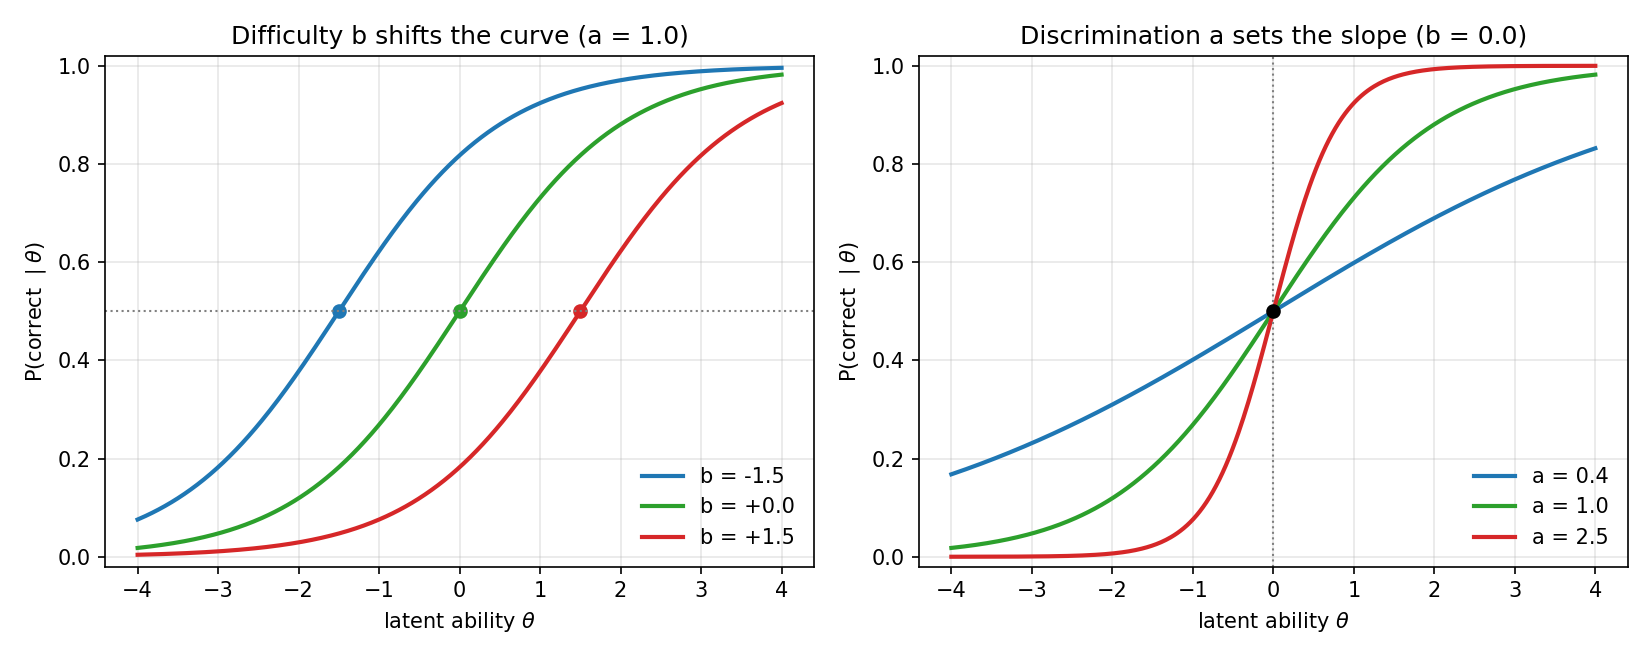
\includegraphics[width=\linewidth]{figures/irt_icc.png}
  \caption{\aiadd{Item characteristic curves for the 2PL model of
  Equation~\eqref{eq:2pl}. Left: difficulty $b$ shifts the sigmoid along the
  ability axis at a fixed discrimination $a = 1$; the dot on each curve marks
  $(\theta = b,\, 0.5)$. Right: discrimination $a$ sets the slope at a fixed
  difficulty $b = 0$, and all three curves cross at $(0,\, 0.5)$. A low-$a$ curve
  rises slowly and separates nearby abilities weakly, while a high-$a$ curve
  rises sharply near $b$.}}
  \label{fig:irt-icc}
\end{figure}

\aibullets{TODO (author): a worked numeric ICC at chosen $a$ and $b$ could help
the reader.}

\subsection{Calibrating the item parameters}

Calibration estimates $a_i$ and $b_i$ for every item from a response matrix, in
which a set of models each answer the items. \aiadd{The standard method is
marginal maximum likelihood with an expectation-maximization (EM) loop, using the
expected item-score counts of Bock and Aitkin~\cite{bock1981marginal} and the
general EM result of Dempster, Laird, and Rubin~\cite{dempster1977maximum}. The
steps below follow the treatment of Baker and Kim~\cite{baker2004item}.}

The loop starts from a prior on ability. We assume $\theta$ is normally
distributed with mean $0$. \aiadd{We fix the variance to $1$ to set the scale,
then replace the continuous prior with a grid of $Q$ quadrature nodes
$X_1 < \cdots < X_Q$ carrying weights $A_1, \dots, A_Q$ that approximate the
normal density and sum to one.} The weights are larger near the center of the
range and small in the tails. \aiadd{A node at $\theta = 0$ therefore carries far
more weight than a node at $\theta = -4$.}

For each model we compute the likelihood of its exact response pattern at every
node. \aiadd{Writing $P_i(X_q) = P(y = 1 \mid X_q, a_i, b_i)$ and assuming local
independence of items given ability, the likelihood of the response pattern
$\mathbf{u}_m = (y_{m1}, \dots, y_{mI})$ of model $m$ at node $X_q$ is}
\begin{equation}
  \aiadd{L(\mathbf{u}_m \mid X_q)
  = \prod_{i=1}^{I} P_i(X_q)^{\,y_{mi}}
    \big(1 - P_i(X_q)\big)^{\,1 - y_{mi}} .}
  \label{eq:pattern-likelihood}
\end{equation}
Each factor is the probability of a correct response where the model answered
correctly, and the probability of a wrong response where it did not.

We multiply these likelihoods by the prior weights, which gives an unnormalized
weight for each model at every node. \aiadd{Normalizing produces a posterior
distribution over the nodes for each model,}
\begin{equation}
  \aiadd{P(X_q \mid \mathbf{u}_m)
  = \frac{L(\mathbf{u}_m \mid X_q)\, A_q}
         {\sum_{q'=1}^{Q} L(\mathbf{u}_m \mid X_{q'})\, A_{q'}} .}
  \label{eq:estep-posterior}
\end{equation}

For each item we then form two expected counts at every node: the expected number
of models at that ability, and the expected number of models at that ability that
answered the item correctly. \aiadd{From the posterior weights these are}
\begin{equation}
  \aiadd{\bar{N}_q = \sum_{m=1}^{M} P(X_q \mid \mathbf{u}_m),
  \qquad
  \bar{R}_{iq} = \sum_{m=1}^{M} y_{mi}\, P(X_q \mid \mathbf{u}_m) .}
  \label{eq:expected-counts}
\end{equation}
These are the $N(\theta_j)$ and $R(\theta_j)$ of the notes, one pair per node
$\theta_j$. The ratio $R(\theta_j) / N(\theta_j)$ is the expected proportion
correct at ability $\theta_j$, and these are the points that the item's curve
must fit. \aiadd{With a complete response matrix $\bar{N}_q$ is the same for every
item, so only $\bar{R}_{iq}$ carries the item index $i$.}

The parameters are then updated by fitting the curve to those points with
logistic regression. \aiadd{The M-step maximizes, for each item, the binomial
log-likelihood of $\bar{R}_{iq}$ correct out of $\bar{N}_q$ at each node,}
\begin{equation}
  \aiadd{\ell_i(a_i, b_i)
  = \sum_{q=1}^{Q} \Big[ \bar{R}_{iq} \log P_i(X_q)
    + (\bar{N}_q - \bar{R}_{iq}) \log\big(1 - P_i(X_q)\big) \Big] .}
  \label{eq:mstep}
\end{equation}
\aiadd{Because $P_i$ is logistic in $\theta$ with linear predictor
$a_i(\theta - b_i) = a_i \theta - a_i b_i$, maximizing
Equation~\eqref{eq:mstep} is a weighted logistic regression of the aggregated
correct and wrong counts on the node values $X_q$, with slope $a_i$ and intercept
$-a_i b_i$.}

We then recompute each $P_i$ with the updated parameters and repeat, updating both
the ability distribution and the item parameters. \aiadd{The loop continues until
the item parameters and the marginal log-likelihood stop changing appreciably.}
This is the Bock and Aitkin~\cite{bock1981marginal} EM calibration. See Baker and
Kim~\cite{baker2004item} and Lord~\cite{lord1980applications} for full
treatments, and Birnbaum~\cite{birnbaum1968some} and
Rasch~\cite{rasch1960probabilistic} for the origins of the 2PL and 1PL models.

\aibullets{TODO (author): identifiability and scale fixing (why
$\theta \sim \mathcal{N}(0,1)$ is enough to pin down the metric), and a pointer to
how the calibrated $a_i, b_i$ feed Fisher-information item selection in the CAT
loop.}

%
% Requires (acmart already loads amsmath, graphicx, natbib, xcolor):
%   \usepackage{amsmath,amssymb,graphicx,xcolor}
% The figure is referenced as figures/irt_icc.png, so compile from the
% _paper_build/ root or add that folder to \graphicspath.
%
% Authoring convention for this draft (matches the sibling section files):
%   \aiadd{...}     AI-written correction or addition, shown in blue.
%   \aibullets{...} blue stub text marking a block of new AI-drafted prose for
%                   the human author to review or expand.
% The surrounding black text is the human author's notes, lightly cleaned.
% ============================================================================

\providecommand{\aiadd}[1]{\textcolor{blue}{#1}}
\providecommand{\aibullets}[1]{{\color{blue}#1}}

\section{Unidimensional IRT Calibration Fundamentals}
\label{app:irt-unidim}

The goal of Item Response Theory (IRT) is to calibrate a set of parameters for
each item so that a Computerized Adaptive Test (CAT) can use them to distinguish
a model's ability. For the unidimensional case, meaning one ability, we assume
each model has a single latent ability $\theta$. Each item is then described by
the probability of a correct response given a latent ability value, and that
probability follows a sigmoid curve. \aiadd{This curve is the item
characteristic curve (ICC).}

\subsection{The item response function}

Let $y$ be the correctness of a response, with $y = 0$ for a wrong answer and
$y = 1$ for a correct answer. For a single item we model the probability
$P(y = 1 \mid \theta, \text{item parameters})$.

With one parameter, the item has a single location on the $\theta$ axis where a
model moves from being unlikely to being likely to answer correctly. This is the
difficulty $b_i$. With two parameters, the second parameter controls how sharp
that boundary is, which is the discrimination $a_i$. This gives the
two-parameter logistic (2PL) model,
%
% Corrected form of the garbled inline equation in the source notes:
% the discrimination a_i multiplies (theta - b_i) inside the exponent.
%
\begin{equation}
  P(y = 1 \mid \theta, a_i, b_i)
  = \frac{\exp\!\big(a_i (\theta - b_i)\big)}{1 + \exp\!\big(a_i (\theta - b_i)\big)}
  = \frac{1}{1 + \exp\!\big(-a_i (\theta - b_i)\big)} .
  \label{eq:2pl}
\end{equation}
%
\aiadd{Fixing $a_i = 1$, or holding a single discrimination common to all items,
reduces Equation~\eqref{eq:2pl} to the one-parameter logistic (1PL), or Rasch,
model}
\begin{equation}
  \aiadd{P(y = 1 \mid \theta, b_i)
  = \frac{\exp(\theta - b_i)}{1 + \exp(\theta - b_i)} .}
  \label{eq:1pl}
\end{equation}

The difficulty $b_i$ is the location of the curve on the $\theta$ axis: the
ability at which the probability of a correct response equals $0.5$. A larger
$b_i$ shifts the curve to the right, so a higher ability is needed to reach even
odds of success. The discrimination $a_i$ controls how steep the curve is around
$b_i$. \aiadd{At $\theta = b_i$ the slope of the 2PL curve is $a_i/4$, so a
larger $a_i$ makes the change from low to high probability sharper and lets the
item separate models with abilities near $b_i$ more finely.}
Figure~\ref{fig:irt-icc} shows both effects.

\begin{figure}[t]
  \centering
  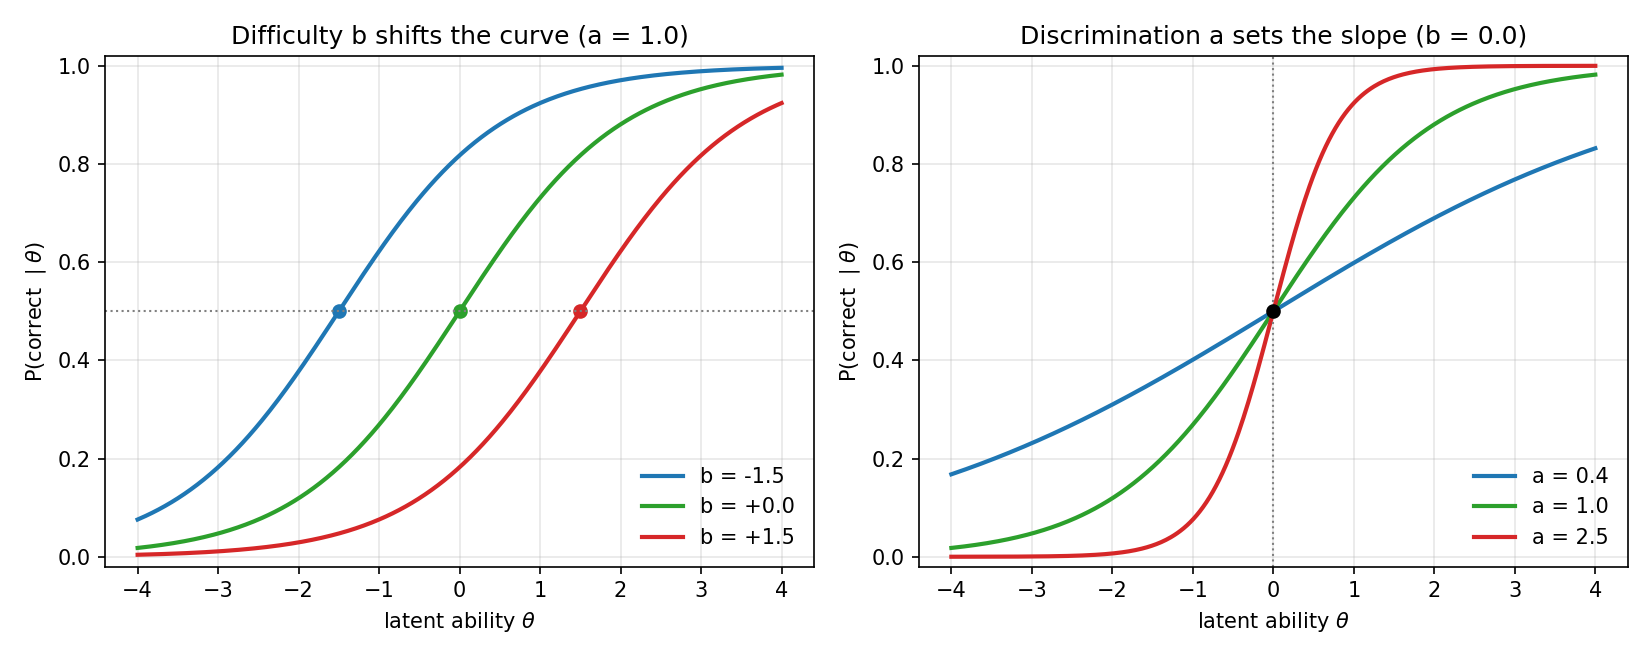
\includegraphics[width=\linewidth]{figures/irt_icc.png}
  \caption{\aiadd{Item characteristic curves for the 2PL model of
  Equation~\eqref{eq:2pl}. Left: difficulty $b$ shifts the sigmoid along the
  ability axis at a fixed discrimination $a = 1$; the dot on each curve marks
  $(\theta = b,\, 0.5)$. Right: discrimination $a$ sets the slope at a fixed
  difficulty $b = 0$, and all three curves cross at $(0,\, 0.5)$. A low-$a$ curve
  rises slowly and separates nearby abilities weakly, while a high-$a$ curve
  rises sharply near $b$.}}
  \label{fig:irt-icc}
\end{figure}

\aibullets{TODO (author): a worked numeric ICC at chosen $a$ and $b$ could help
the reader.}

\subsection{Calibrating the item parameters}

Calibration estimates $a_i$ and $b_i$ for every item from a response matrix, in
which a set of models each answer the items. \aiadd{The standard method is
marginal maximum likelihood with an expectation-maximization (EM) loop, using the
expected item-score counts of Bock and Aitkin~\cite{bock1981marginal} and the
general EM result of Dempster, Laird, and Rubin~\cite{dempster1977maximum}. The
steps below follow the treatment of Baker and Kim~\cite{baker2004item}.}

The loop starts from a prior on ability. We assume $\theta$ is normally
distributed with mean $0$. \aiadd{We fix the variance to $1$ to set the scale,
then replace the continuous prior with a grid of $Q$ quadrature nodes
$X_1 < \cdots < X_Q$ carrying weights $A_1, \dots, A_Q$ that approximate the
normal density and sum to one.} The weights are larger near the center of the
range and small in the tails. \aiadd{A node at $\theta = 0$ therefore carries far
more weight than a node at $\theta = -4$.}

For each model we compute the likelihood of its exact response pattern at every
node. \aiadd{Writing $P_i(X_q) = P(y = 1 \mid X_q, a_i, b_i)$ and assuming local
independence of items given ability, the likelihood of the response pattern
$\mathbf{u}_m = (y_{m1}, \dots, y_{mI})$ of model $m$ at node $X_q$ is}
\begin{equation}
  \aiadd{L(\mathbf{u}_m \mid X_q)
  = \prod_{i=1}^{I} P_i(X_q)^{\,y_{mi}}
    \big(1 - P_i(X_q)\big)^{\,1 - y_{mi}} .}
  \label{eq:pattern-likelihood}
\end{equation}
Each factor is the probability of a correct response where the model answered
correctly, and the probability of a wrong response where it did not.

We multiply these likelihoods by the prior weights, which gives an unnormalized
weight for each model at every node. \aiadd{Normalizing produces a posterior
distribution over the nodes for each model,}
\begin{equation}
  \aiadd{P(X_q \mid \mathbf{u}_m)
  = \frac{L(\mathbf{u}_m \mid X_q)\, A_q}
         {\sum_{q'=1}^{Q} L(\mathbf{u}_m \mid X_{q'})\, A_{q'}} .}
  \label{eq:estep-posterior}
\end{equation}

For each item we then form two expected counts at every node: the expected number
of models at that ability, and the expected number of models at that ability that
answered the item correctly. \aiadd{From the posterior weights these are}
\begin{equation}
  \aiadd{\bar{N}_q = \sum_{m=1}^{M} P(X_q \mid \mathbf{u}_m),
  \qquad
  \bar{R}_{iq} = \sum_{m=1}^{M} y_{mi}\, P(X_q \mid \mathbf{u}_m) .}
  \label{eq:expected-counts}
\end{equation}
These are the $N(\theta_j)$ and $R(\theta_j)$ of the notes, one pair per node
$\theta_j$. The ratio $R(\theta_j) / N(\theta_j)$ is the expected proportion
correct at ability $\theta_j$, and these are the points that the item's curve
must fit. \aiadd{With a complete response matrix $\bar{N}_q$ is the same for every
item, so only $\bar{R}_{iq}$ carries the item index $i$.}

The parameters are then updated by fitting the curve to those points with
logistic regression. \aiadd{The M-step maximizes, for each item, the binomial
log-likelihood of $\bar{R}_{iq}$ correct out of $\bar{N}_q$ at each node,}
\begin{equation}
  \aiadd{\ell_i(a_i, b_i)
  = \sum_{q=1}^{Q} \Big[ \bar{R}_{iq} \log P_i(X_q)
    + (\bar{N}_q - \bar{R}_{iq}) \log\big(1 - P_i(X_q)\big) \Big] .}
  \label{eq:mstep}
\end{equation}
\aiadd{Because $P_i$ is logistic in $\theta$ with linear predictor
$a_i(\theta - b_i) = a_i \theta - a_i b_i$, maximizing
Equation~\eqref{eq:mstep} is a weighted logistic regression of the aggregated
correct and wrong counts on the node values $X_q$, with slope $a_i$ and intercept
$-a_i b_i$.}

We then recompute each $P_i$ with the updated parameters and repeat, updating both
the ability distribution and the item parameters. \aiadd{The loop continues until
the item parameters and the marginal log-likelihood stop changing appreciably.}
This is the Bock and Aitkin~\cite{bock1981marginal} EM calibration. See Baker and
Kim~\cite{baker2004item} and Lord~\cite{lord1980applications} for full
treatments, and Birnbaum~\cite{birnbaum1968some} and
Rasch~\cite{rasch1960probabilistic} for the origins of the 2PL and 1PL models.

\aibullets{TODO (author): identifiability and scale fixing (why
$\theta \sim \mathcal{N}(0,1)$ is enough to pin down the metric), and a pointer to
how the calibrated $a_i, b_i$ feed Fisher-information item selection in the CAT
loop.}

%
% Requires (acmart already loads amsmath, graphicx, natbib, xcolor):
%   \usepackage{amsmath,amssymb,graphicx,xcolor}
% The figure is referenced as figures/irt_icc.png, so compile from the
% _paper_build/ root or add that folder to \graphicspath.
%
% Authoring convention for this draft (matches the sibling section files):
%   \aiadd{...}     AI-written correction or addition, shown in blue.
%   \aibullets{...} blue stub text marking a block of new AI-drafted prose for
%                   the human author to review or expand.
% The surrounding black text is the human author's notes, lightly cleaned.
% ============================================================================

\providecommand{\aiadd}[1]{\textcolor{blue}{#1}}
\providecommand{\aibullets}[1]{{\color{blue}#1}}

\section{Unidimensional IRT Calibration Fundamentals}
\label{app:irt-unidim}

The goal of Item Response Theory (IRT) is to calibrate a set of parameters for
each item so that a Computerized Adaptive Test (CAT) can use them to distinguish
a model's ability. For the unidimensional case, meaning one ability, we assume
each model has a single latent ability $\theta$. Each item is then described by
the probability of a correct response given a latent ability value, and that
probability follows a sigmoid curve. \aiadd{This curve is the item
characteristic curve (ICC).}

\subsection{The item response function}

Let $y$ be the correctness of a response, with $y = 0$ for a wrong answer and
$y = 1$ for a correct answer. For a single item we model the probability
$P(y = 1 \mid \theta, \text{item parameters})$.

With one parameter, the item has a single location on the $\theta$ axis where a
model moves from being unlikely to being likely to answer correctly. This is the
difficulty $b_i$. With two parameters, the second parameter controls how sharp
that boundary is, which is the discrimination $a_i$. This gives the
two-parameter logistic (2PL) model,
%
% Corrected form of the garbled inline equation in the source notes:
% the discrimination a_i multiplies (theta - b_i) inside the exponent.
%
\begin{equation}
  P(y = 1 \mid \theta, a_i, b_i)
  = \frac{\exp\!\big(a_i (\theta - b_i)\big)}{1 + \exp\!\big(a_i (\theta - b_i)\big)}
  = \frac{1}{1 + \exp\!\big(-a_i (\theta - b_i)\big)} .
  \label{eq:2pl}
\end{equation}
%
\aiadd{Fixing $a_i = 1$, or holding a single discrimination common to all items,
reduces Equation~\eqref{eq:2pl} to the one-parameter logistic (1PL), or Rasch,
model}
\begin{equation}
  \aiadd{P(y = 1 \mid \theta, b_i)
  = \frac{\exp(\theta - b_i)}{1 + \exp(\theta - b_i)} .}
  \label{eq:1pl}
\end{equation}

The difficulty $b_i$ is the location of the curve on the $\theta$ axis: the
ability at which the probability of a correct response equals $0.5$. A larger
$b_i$ shifts the curve to the right, so a higher ability is needed to reach even
odds of success. The discrimination $a_i$ controls how steep the curve is around
$b_i$. \aiadd{At $\theta = b_i$ the slope of the 2PL curve is $a_i/4$, so a
larger $a_i$ makes the change from low to high probability sharper and lets the
item separate models with abilities near $b_i$ more finely.}
Figure~\ref{fig:irt-icc} shows both effects.

\begin{figure}[t]
  \centering
  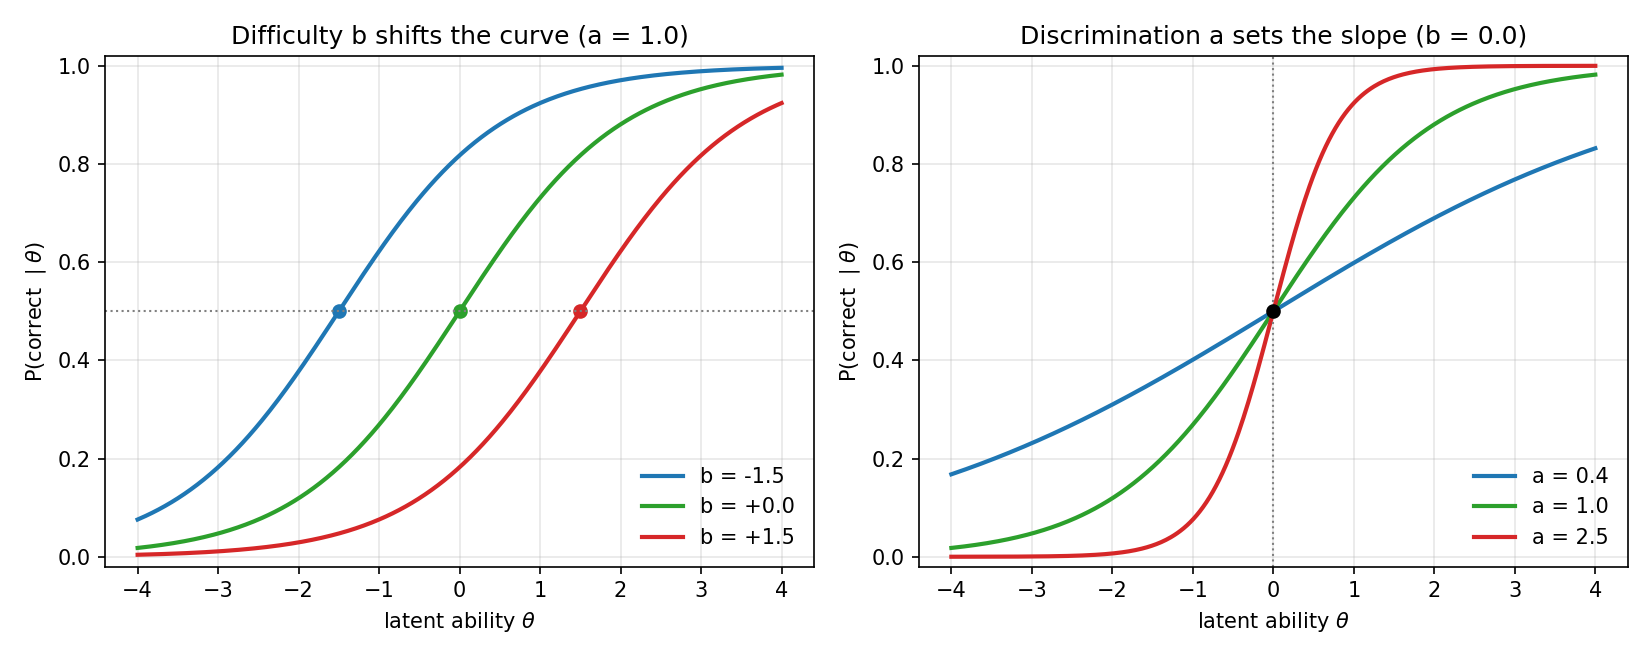
\includegraphics[width=\linewidth]{figures/irt_icc.png}
  \caption{\aiadd{Item characteristic curves for the 2PL model of
  Equation~\eqref{eq:2pl}. Left: difficulty $b$ shifts the sigmoid along the
  ability axis at a fixed discrimination $a = 1$; the dot on each curve marks
  $(\theta = b,\, 0.5)$. Right: discrimination $a$ sets the slope at a fixed
  difficulty $b = 0$, and all three curves cross at $(0,\, 0.5)$. A low-$a$ curve
  rises slowly and separates nearby abilities weakly, while a high-$a$ curve
  rises sharply near $b$.}}
  \label{fig:irt-icc}
\end{figure}

\aibullets{TODO (author): a worked numeric ICC at chosen $a$ and $b$ could help
the reader.}

\subsection{Calibrating the item parameters}

Calibration estimates $a_i$ and $b_i$ for every item from a response matrix, in
which a set of models each answer the items. \aiadd{The standard method is
marginal maximum likelihood with an expectation-maximization (EM) loop, using the
expected item-score counts of Bock and Aitkin~\cite{bock1981marginal} and the
general EM result of Dempster, Laird, and Rubin~\cite{dempster1977maximum}. The
steps below follow the treatment of Baker and Kim~\cite{baker2004item}.}

The loop starts from a prior on ability. We assume $\theta$ is normally
distributed with mean $0$. \aiadd{We fix the variance to $1$ to set the scale,
then replace the continuous prior with a grid of $Q$ quadrature nodes
$X_1 < \cdots < X_Q$ carrying weights $A_1, \dots, A_Q$ that approximate the
normal density and sum to one.} The weights are larger near the center of the
range and small in the tails. \aiadd{A node at $\theta = 0$ therefore carries far
more weight than a node at $\theta = -4$.}

For each model we compute the likelihood of its exact response pattern at every
node. \aiadd{Writing $P_i(X_q) = P(y = 1 \mid X_q, a_i, b_i)$ and assuming local
independence of items given ability, the likelihood of the response pattern
$\mathbf{u}_m = (y_{m1}, \dots, y_{mI})$ of model $m$ at node $X_q$ is}
\begin{equation}
  \aiadd{L(\mathbf{u}_m \mid X_q)
  = \prod_{i=1}^{I} P_i(X_q)^{\,y_{mi}}
    \big(1 - P_i(X_q)\big)^{\,1 - y_{mi}} .}
  \label{eq:pattern-likelihood}
\end{equation}
Each factor is the probability of a correct response where the model answered
correctly, and the probability of a wrong response where it did not.

We multiply these likelihoods by the prior weights, which gives an unnormalized
weight for each model at every node. \aiadd{Normalizing produces a posterior
distribution over the nodes for each model,}
\begin{equation}
  \aiadd{P(X_q \mid \mathbf{u}_m)
  = \frac{L(\mathbf{u}_m \mid X_q)\, A_q}
         {\sum_{q'=1}^{Q} L(\mathbf{u}_m \mid X_{q'})\, A_{q'}} .}
  \label{eq:estep-posterior}
\end{equation}

For each item we then form two expected counts at every node: the expected number
of models at that ability, and the expected number of models at that ability that
answered the item correctly. \aiadd{From the posterior weights these are}
\begin{equation}
  \aiadd{\bar{N}_q = \sum_{m=1}^{M} P(X_q \mid \mathbf{u}_m),
  \qquad
  \bar{R}_{iq} = \sum_{m=1}^{M} y_{mi}\, P(X_q \mid \mathbf{u}_m) .}
  \label{eq:expected-counts}
\end{equation}
These are the $N(\theta_j)$ and $R(\theta_j)$ of the notes, one pair per node
$\theta_j$. The ratio $R(\theta_j) / N(\theta_j)$ is the expected proportion
correct at ability $\theta_j$, and these are the points that the item's curve
must fit. \aiadd{With a complete response matrix $\bar{N}_q$ is the same for every
item, so only $\bar{R}_{iq}$ carries the item index $i$.}

The parameters are then updated by fitting the curve to those points with
logistic regression. \aiadd{The M-step maximizes, for each item, the binomial
log-likelihood of $\bar{R}_{iq}$ correct out of $\bar{N}_q$ at each node,}
\begin{equation}
  \aiadd{\ell_i(a_i, b_i)
  = \sum_{q=1}^{Q} \Big[ \bar{R}_{iq} \log P_i(X_q)
    + (\bar{N}_q - \bar{R}_{iq}) \log\big(1 - P_i(X_q)\big) \Big] .}
  \label{eq:mstep}
\end{equation}
\aiadd{Because $P_i$ is logistic in $\theta$ with linear predictor
$a_i(\theta - b_i) = a_i \theta - a_i b_i$, maximizing
Equation~\eqref{eq:mstep} is a weighted logistic regression of the aggregated
correct and wrong counts on the node values $X_q$, with slope $a_i$ and intercept
$-a_i b_i$.}

We then recompute each $P_i$ with the updated parameters and repeat, updating both
the ability distribution and the item parameters. \aiadd{The loop continues until
the item parameters and the marginal log-likelihood stop changing appreciably.}
This is the Bock and Aitkin~\cite{bock1981marginal} EM calibration. See Baker and
Kim~\cite{baker2004item} and Lord~\cite{lord1980applications} for full
treatments, and Birnbaum~\cite{birnbaum1968some} and
Rasch~\cite{rasch1960probabilistic} for the origins of the 2PL and 1PL models.

\aibullets{TODO (author): identifiability and scale fixing (why
$\theta \sim \mathcal{N}(0,1)$ is enough to pin down the metric), and a pointer to
how the calibrated $a_i, b_i$ feed Fisher-information item selection in the CAT
loop.}

%
% Requires (acmart already loads amsmath, graphicx, natbib, xcolor):
%   \usepackage{amsmath,amssymb,graphicx,xcolor}
% The figure is referenced as figures/irt_icc.png, so compile from the
% _paper_build/ root or add that folder to \graphicspath.
%
% Authoring convention for this draft (matches the sibling section files):
%   \aiadd{...}     AI-written correction or addition, shown in blue.
%   \aibullets{...} blue stub text marking a block of new AI-drafted prose for
%                   the human author to review or expand.
% The surrounding black text is the human author's notes, lightly cleaned.
% ============================================================================

\providecommand{\aiadd}[1]{\textcolor{blue}{#1}}
\providecommand{\aibullets}[1]{{\color{blue}#1}}

\section{Unidimensional IRT Calibration Fundamentals}
\label{app:irt-unidim}

The goal of Item Response Theory (IRT) is to calibrate a set of parameters for
each item so that a Computerized Adaptive Test (CAT) can use them to distinguish
a model's ability. For the unidimensional case, meaning one ability, we assume
each model has a single latent ability $\theta$. Each item is then described by
the probability of a correct response given a latent ability value, and that
probability follows a sigmoid curve. \aiadd{This curve is the item
characteristic curve (ICC).}

\subsection{The item response function}

Let $y$ be the correctness of a response, with $y = 0$ for a wrong answer and
$y = 1$ for a correct answer. For a single item we model the probability
$P(y = 1 \mid \theta, \text{item parameters})$.

With one parameter, the item has a single location on the $\theta$ axis where a
model moves from being unlikely to being likely to answer correctly. This is the
difficulty $b_i$. With two parameters, the second parameter controls how sharp
that boundary is, which is the discrimination $a_i$. This gives the
two-parameter logistic (2PL) model,
%
% Corrected form of the garbled inline equation in the source notes:
% the discrimination a_i multiplies (theta - b_i) inside the exponent.
%
\begin{equation}
  P(y = 1 \mid \theta, a_i, b_i)
  = \frac{\exp\!\big(a_i (\theta - b_i)\big)}{1 + \exp\!\big(a_i (\theta - b_i)\big)}
  = \frac{1}{1 + \exp\!\big(-a_i (\theta - b_i)\big)} .
  \label{eq:2pl}
\end{equation}
%
\aiadd{Fixing $a_i = 1$, or holding a single discrimination common to all items,
reduces Equation~\eqref{eq:2pl} to the one-parameter logistic (1PL), or Rasch,
model}
\begin{equation}
  \aiadd{P(y = 1 \mid \theta, b_i)
  = \frac{\exp(\theta - b_i)}{1 + \exp(\theta - b_i)} .}
  \label{eq:1pl}
\end{equation}

The difficulty $b_i$ is the location of the curve on the $\theta$ axis: the
ability at which the probability of a correct response equals $0.5$. A larger
$b_i$ shifts the curve to the right, so a higher ability is needed to reach even
odds of success. The discrimination $a_i$ controls how steep the curve is around
$b_i$. \aiadd{At $\theta = b_i$ the slope of the 2PL curve is $a_i/4$, so a
larger $a_i$ makes the change from low to high probability sharper and lets the
item separate models with abilities near $b_i$ more finely.}
Figure~\ref{fig:irt-icc} shows both effects.

\begin{figure}[t]
  \centering
  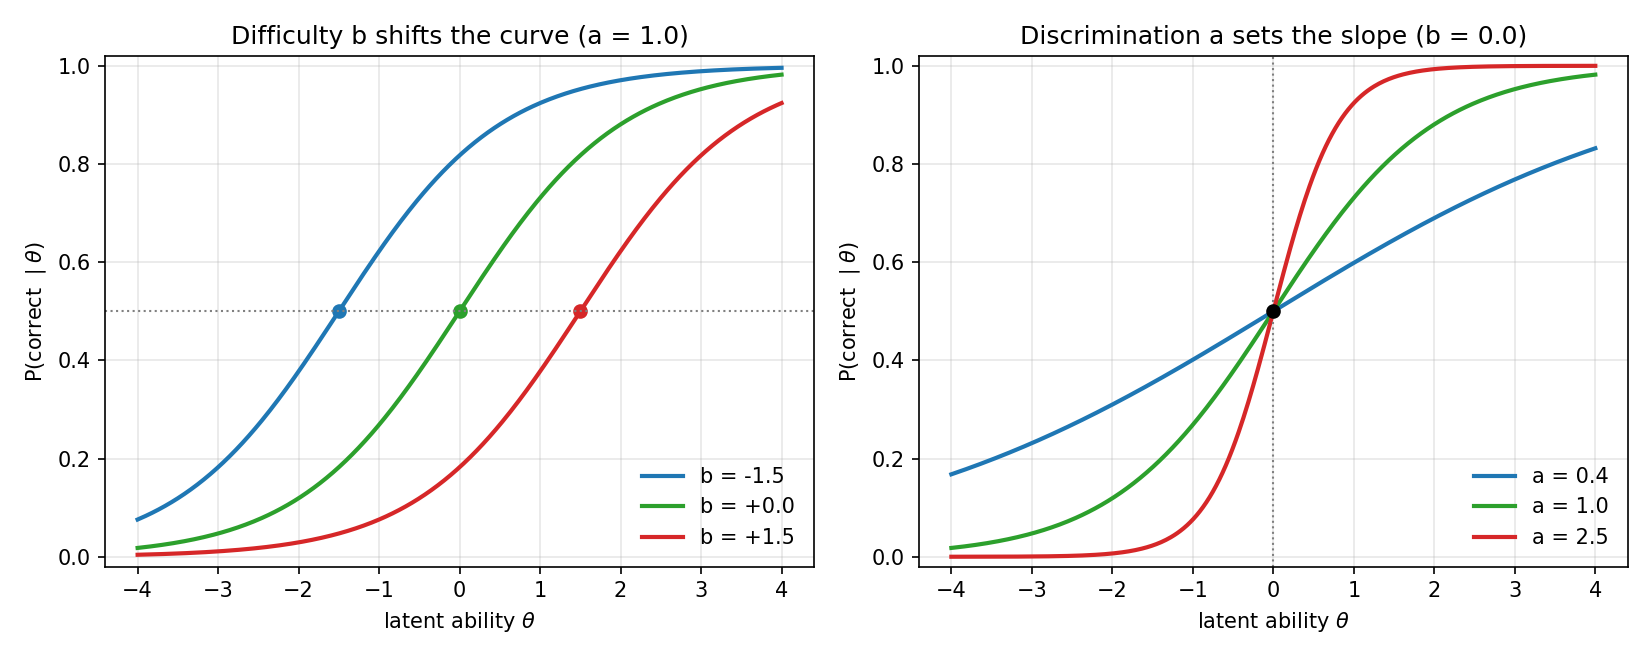
\includegraphics[width=\linewidth]{figures/irt_icc.png}
  \caption{\aiadd{Item characteristic curves for the 2PL model of
  Equation~\eqref{eq:2pl}. Left: difficulty $b$ shifts the sigmoid along the
  ability axis at a fixed discrimination $a = 1$; the dot on each curve marks
  $(\theta = b,\, 0.5)$. Right: discrimination $a$ sets the slope at a fixed
  difficulty $b = 0$, and all three curves cross at $(0,\, 0.5)$. A low-$a$ curve
  rises slowly and separates nearby abilities weakly, while a high-$a$ curve
  rises sharply near $b$.}}
  \label{fig:irt-icc}
\end{figure}

\aibullets{TODO (author): a worked numeric ICC at chosen $a$ and $b$ could help
the reader.}

\subsection{Calibrating the item parameters}

Calibration estimates $a_i$ and $b_i$ for every item from a response matrix, in
which a set of models each answer the items. \aiadd{The standard method is
marginal maximum likelihood with an expectation-maximization (EM) loop, using the
expected item-score counts of Bock and Aitkin~\cite{bock1981marginal} and the
general EM result of Dempster, Laird, and Rubin~\cite{dempster1977maximum}. The
steps below follow the treatment of Baker and Kim~\cite{baker2004item}.}

The loop starts from a prior on ability. We assume $\theta$ is normally
distributed with mean $0$. \aiadd{We fix the variance to $1$ to set the scale,
then replace the continuous prior with a grid of $Q$ quadrature nodes
$X_1 < \cdots < X_Q$ carrying weights $A_1, \dots, A_Q$ that approximate the
normal density and sum to one.} The weights are larger near the center of the
range and small in the tails. \aiadd{A node at $\theta = 0$ therefore carries far
more weight than a node at $\theta = -4$.}

For each model we compute the likelihood of its exact response pattern at every
node. \aiadd{Writing $P_i(X_q) = P(y = 1 \mid X_q, a_i, b_i)$ and assuming local
independence of items given ability, the likelihood of the response pattern
$\mathbf{u}_m = (y_{m1}, \dots, y_{mI})$ of model $m$ at node $X_q$ is}
\begin{equation}
  \aiadd{L(\mathbf{u}_m \mid X_q)
  = \prod_{i=1}^{I} P_i(X_q)^{\,y_{mi}}
    \big(1 - P_i(X_q)\big)^{\,1 - y_{mi}} .}
  \label{eq:pattern-likelihood}
\end{equation}
Each factor is the probability of a correct response where the model answered
correctly, and the probability of a wrong response where it did not.

We multiply these likelihoods by the prior weights, which gives an unnormalized
weight for each model at every node. \aiadd{Normalizing produces a posterior
distribution over the nodes for each model,}
\begin{equation}
  \aiadd{P(X_q \mid \mathbf{u}_m)
  = \frac{L(\mathbf{u}_m \mid X_q)\, A_q}
         {\sum_{q'=1}^{Q} L(\mathbf{u}_m \mid X_{q'})\, A_{q'}} .}
  \label{eq:estep-posterior}
\end{equation}

For each item we then form two expected counts at every node: the expected number
of models at that ability, and the expected number of models at that ability that
answered the item correctly. \aiadd{From the posterior weights these are}
\begin{equation}
  \aiadd{\bar{N}_q = \sum_{m=1}^{M} P(X_q \mid \mathbf{u}_m),
  \qquad
  \bar{R}_{iq} = \sum_{m=1}^{M} y_{mi}\, P(X_q \mid \mathbf{u}_m) .}
  \label{eq:expected-counts}
\end{equation}
These are the $N(\theta_j)$ and $R(\theta_j)$ of the notes, one pair per node
$\theta_j$. The ratio $R(\theta_j) / N(\theta_j)$ is the expected proportion
correct at ability $\theta_j$, and these are the points that the item's curve
must fit. \aiadd{With a complete response matrix $\bar{N}_q$ is the same for every
item, so only $\bar{R}_{iq}$ carries the item index $i$.}

The parameters are then updated by fitting the curve to those points with
logistic regression. \aiadd{The M-step maximizes, for each item, the binomial
log-likelihood of $\bar{R}_{iq}$ correct out of $\bar{N}_q$ at each node,}
\begin{equation}
  \aiadd{\ell_i(a_i, b_i)
  = \sum_{q=1}^{Q} \Big[ \bar{R}_{iq} \log P_i(X_q)
    + (\bar{N}_q - \bar{R}_{iq}) \log\big(1 - P_i(X_q)\big) \Big] .}
  \label{eq:mstep}
\end{equation}
\aiadd{Because $P_i$ is logistic in $\theta$ with linear predictor
$a_i(\theta - b_i) = a_i \theta - a_i b_i$, maximizing
Equation~\eqref{eq:mstep} is a weighted logistic regression of the aggregated
correct and wrong counts on the node values $X_q$, with slope $a_i$ and intercept
$-a_i b_i$.}

We then recompute each $P_i$ with the updated parameters and repeat, updating both
the ability distribution and the item parameters. \aiadd{The loop continues until
the item parameters and the marginal log-likelihood stop changing appreciably.}
This is the Bock and Aitkin~\cite{bock1981marginal} EM calibration. See Baker and
Kim~\cite{baker2004item} and Lord~\cite{lord1980applications} for full
treatments, and Birnbaum~\cite{birnbaum1968some} and
Rasch~\cite{rasch1960probabilistic} for the origins of the 2PL and 1PL models.

\aibullets{TODO (author): identifiability and scale fixing (why
$\theta \sim \mathcal{N}(0,1)$ is enough to pin down the metric), and a pointer to
how the calibrated $a_i, b_i$ feed Fisher-information item selection in the CAT
loop.}
